%% =====================================================================
%%  VL401: RTL Design and Verification -- Course Project Report
%%  Group 07, Project P07: Real-Time Edge-Detection Video Pipeline
%%  Built from the course template (VL401_Report_Template.tex).  Compile: pdflatex x2
%% =====================================================================
\documentclass[11pt,a4paper]{article}

\usepackage[T1]{fontenc}
\usepackage[utf8]{inputenc}
\IfFileExists{lmodern.sty}{\usepackage{lmodern}}{}
\usepackage[margin=2.2cm]{geometry}
\usepackage{amsmath,amssymb}
\usepackage{graphicx}
\usepackage{booktabs,tabularx,multirow,array}
\usepackage[table]{xcolor}
\usepackage{enumitem}
\usepackage{listings}
\usepackage{caption}
\usepackage{float}
\usepackage{fancyhdr}
\usepackage{tikz}
\usetikzlibrary{arrows.meta,positioning,shapes,fit,calc}
\usepackage[colorlinks=true,linkcolor=blue!50!black,citecolor=blue!50!black,urlcolor=blue!50!black]{hyperref}

%% =====================================================================
%%  GROUP DETAILS
%% =====================================================================
\newcommand{\groupno}{07}
\newcommand{\projno}{P07}
\newcommand{\projtitle}{Real-Time Edge-Detection Video Pipeline}
\newcommand{\studentA}{Gundoju Sai Vamshi}
\newcommand{\rollA}{B23263}
\newcommand{\studentB}{Shashank Tiwari}
\newcommand{\rollB}{B24499}
\newcommand{\repourl}{https://github.com/vamshi-246/vision}
\newcommand{\submitdate}{November 24, 2026}

\newif\ifguidance
\guidancefalse

\definecolor{iitblue}{RGB}{0,51,102}
\definecolor{guidebg}{RGB}{232,240,252}
\newcommand{\guide}[1]{\ifguidance\par\noindent
  \colorbox{guidebg}{\parbox{\dimexpr\linewidth-2\fboxsep}{\small\itshape
  \textbf{Guidance:} #1}}\par\medskip\fi}

\newcommand{\figfile}[4]{%
\begin{figure}[H]\centering
\IfFileExists{#1}{\includegraphics[width=#2]{#1}}%
{\fbox{\parbox[c][4cm][c]{#2}{\centering\color{gray}\small
  [Placeholder: put \texttt{\detokenize{#1}} in this folder]}}}
\caption{#3}\label{#4}
\end{figure}}

\lstdefinelanguage{SMV}{morekeywords={MODULE,VAR,IVAR,ASSIGN,DEFINE,INIT,INVAR,init,next,case,esac,
  SPEC,CTLSPEC,LTLSPEC,FAIRNESS,boolean,AG,AF,AX,EG,EF,EX,A,E,U,TRUE,FALSE},
  sensitive=true,morecomment=[l]{--}}
\lstset{basicstyle=\ttfamily\footnotesize,keywordstyle=\color{iitblue}\bfseries,
  commentstyle=\color{gray}\itshape,numbers=left,numberstyle=\tiny\color{gray},
  frame=single,rulecolor=\color{gray!50},breaklines=true,columns=fullflexible,
  captionpos=b,xleftmargin=1.5em,framexleftmargin=1.2em}

\setlength{\parskip}{2pt}
\setlength{\emergencystretch}{3em}
\setlength{\parindent}{0pt}
\setlist{nosep,leftmargin=1.4em}
\setlength{\textfloatsep}{8pt plus 2pt}
\setlength{\floatsep}{6pt plus 2pt}
\setlength{\intextsep}{6pt plus 2pt}
\captionsetup{font=small,skip=3pt}

\pagestyle{fancy}
\fancyhf{}
\lhead{\small VL401 Course Project -- Group \groupno}
\rhead{\small \projno: \projtitle}
\cfoot{\small \thepage}

\begin{document}

%% =====================================================================
\begin{titlepage}
\centering
{\large Indian Institute of Technology Mandi}\\[2pt]
{\normalsize School of Computing and Electrical Engineering}\\[1.6cm]
{\Large\bfseries VL401: RTL Design and Verification}\\[4pt]
{\large Course Project Report -- Odd Semester 2026}\\[1.6cm]
{\color{iitblue}\rule{\linewidth}{1pt}}\\[8pt]
{\LARGE\bfseries \projno: \projtitle}\\[8pt]
{\color{iitblue}\rule{\linewidth}{1pt}}\\[1.4cm]
{\large Group \groupno}\\[10pt]
\begin{tabular}{ll}
\toprule
\textbf{Name} & \textbf{Roll No.}\\
\midrule
\studentA & \rollA\\
\studentB & \rollB\\
\bottomrule
\end{tabular}\\[1.2cm]
\begin{tabular}{rl}
Instructor: & Dr.\ Bikram Paul\\
Repository: & \url{\repourl}\\
Submitted on: & \submitdate\\
\end{tabular}
\vfill
\begin{minipage}{0.92\linewidth}\small
\textbf{Declaration.} We declare that the RTL, verification code and analysis in this report are our own
work, except where sources (including open-source IP and AI tools) are acknowledged in
Section~\ref{sec:contrib}.\\[1.0cm]
\rule{5.5cm}{0.4pt}\hfill\rule{5.5cm}{0.4pt}\\
\studentA\hfill\studentB
\end{minipage}
\end{titlepage}

%% =====================================================================
\begin{abstract}
Edge detection is the first step of most machine-vision systems, and on video it must keep up with the pixel rate.
We designed a streaming Canny-style edge detector for 640$\times$480 video at 60\,Hz, one pixel per clock:
3$\times$3 Gaussian, Sobel $|G_x|+|G_y|$ with a quantised direction, non-maximum suppression (NMS) and a double threshold.
The Sobel datapath was derived by hand HLS (all 22 multiplications removed,
critical path from 12 to 7 steps); the direction/NMS-select logic was minimised with ESPRESSO, our own Quine--McCluskey
solver and BDDs. A PicoRV32 core reads the edge count and histogram over APB and sets the thresholds.
From Guo and Wu we took an adaptive Otsu threshold. Their design needs a frame buffer larger than our FPGA; our
streaming version needs one extra BRAM tile and gives the same thresholds on six test images.
The RTL matches a Python golden model on 29.8 million pixels and is checked by 13 SVA assertions, 25 CTL properties in
NuSMV and SymbiYosys k-induction. On a Zybo Z7-10 it meets timing at 25.18\,MHz, uses 3 BRAM tiles and no DSP in the core,
runs live webcam video over HDMI, and is 437$\times$ faster than software on the RV32 core.
\end{abstract}

\tableofcontents
\newpage

%% =====================================================================
\section{Introduction}
\label{sec:intro}
Edges (sharp changes of brightness) carry most of the structure of an image; lane detection, document scanning,
industrial inspection and object recognition all start from an edge map. The Canny detector~\cite{canny} is the
standard method, but it is sequential (smooth, differentiate, thin, threshold) and touches every pixel several times,
so a software implementation on a small processor cannot keep up with video. An FPGA can, because every stage is a
3$\times$3 neighbourhood operation that can be pipelined: with two line buffers per stage, one new pixel enters and one
classified pixel leaves every clock, with a latency of only a few lines and no frame buffer.

\subsection{Objectives}
\begin{enumerate}
  \item Build a streaming edge pipeline (Gaussian $\rightarrow$ Sobel magnitude and direction $\rightarrow$ NMS
  $\rightarrow$ double threshold) for 640$\times$480@60\,Hz at one pixel per clock, bit-exact with a Python golden model.
  \item Derive the Sobel datapath by hand HLS; minimise the direction/NMS-select logic (ESPRESSO, QM, BDD).
  \item Integrate it with a VGA-timed display path, an APB register bank and an RV32 core that reads statistics.
  \item Verify it by simulation (golden-model scoreboards, assertions, coverage) and formally (CTL, BDD, SymbiYosys).
  \item Incorporate an adaptive-threshold technique from the literature and compare resources and quality.
  \item Demonstrate it live on the Zybo Z7-10: switch between original, smoothed and edge views; thresholds from switches.
\end{enumerate}
\textbf{Achieved.} All objectives were met (the paper-based unit in simulation and synthesis only), with two substitutions explained in Section~\ref{sec:discussion}: the
display is VGA-timed 640$\times$480 carried over HDMI/DVI (the Z7-10 has no VGA connector), and frames come from on-chip BRAM
loaded over JTAG, or live from a laptop webcam over HDMI-in, instead of DDR/DMA and an OV7670 camera.
Section~\ref{sec:related} reviews the background and the chosen paper; Sections~\ref{sec:spec}--\ref{sec:fpga} follow the design
flow from specification to FPGA; Sections~\ref{sec:discussion} and \ref{sec:conclusion} discuss limits and conclude.

%% =====================================================================
\section{Background and Related Work}
\label{sec:related}
\subsection{Background}
\textbf{Canny pipeline.} Canny~\cite{canny} smooths with a Gaussian, computes the gradient, keeps only local maxima along the
gradient direction (NMS) and classifies survivors with two thresholds: \emph{strong} ($\ge T_\text{hi}$) and \emph{weak}
($\ge T_\text{lo}$). Hardware versions replace the Euclidean magnitude by $|G_x|+|G_y|$ and quantise the direction to four
sectors (0$^\circ$, 45$^\circ$, 90$^\circ$, 135$^\circ$) with comparisons of $|G_x|$ and $|G_y|$ against $\tan 22.5^\circ\approx 13/32$.
\textbf{Video timing.} The display follows the VESA DMT 640$\times$480@60\,Hz format~\cite{vesa}: 800$\times$525 clocks per frame,
25.175\,MHz pixel clock, so the pipeline has exactly one clock per pixel.

\textbf{Related work.} Xu \emph{et al.}~\cite{xu2014} split the image into blocks and compute a threshold per block from the
block's gradient histogram, which needs block buffers. He and Yuan~\cite{he2008} pipeline Canny on an FPGA with a fixed
threshold. Otsu's method~\cite{otsu} picks the threshold that maximises the between-class variance of a histogram and is
the usual basis for adaptive Canny thresholds. Guo and Wu~\cite{guo2023} combine Canny with an Otsu threshold computed in
a division-free, logarithm-domain unit on the FPGA; this is the paper we chose. It matches the research option
``adaptive-threshold Canny on FPGA'' on our project card, and it lets us compare the gain in output quality with the extra
hardware it needs.

\subsection{Chosen Paper and Paper-to-RTL Plan}
\begin{table}[H]\centering\footnotesize
\caption{Paper-to-RTL contract.}\label{tab:contract}
\begin{tabularx}{\linewidth}{@{}lX@{}}
\toprule
Paper & L. Guo and S. Wu, ``FPGA implementation of a real-time edge detection system based on an improved Canny algorithm,''
\emph{Applied Sciences}, vol.~13, no.~2, art.~870, 2023, doi:10.3390/app13020870~\cite{guo2023}.\\
Technique & $T_\text{hi}$ is chosen per frame by Otsu's method on a 256-bin histogram of the 8-bit-saturated NMS magnitude,
evaluated without division as $2\log_2|s_0N-Sw_0|-\log_2 w_0-\log_2 w_1$; $T_\text{lo}=T_\text{hi}/2$.\\
Claim to reproduce & An adaptive threshold that follows the image content, giving better edge maps than a fixed threshold,
in real time on an FPGA.\\
Block affected & Classifier thresholds (\texttt{classify\_hist}); new histogram + Otsu unit (\texttt{otsu\_stream}, \texttt{otsu\_ctrl}).\\
Baseline & Our streaming core with fixed thresholds 64/192, and a plain Sobel $\ge$192 detector.\\
Metrics & LUT/FF/BRAM/DSP and $F_\text{max}$ (Vivado, same device, same 10\,ns OOC flow); threshold equality with the
paper's engine; PSNR and F1 against the golden map and scikit-image Canny.\\
\bottomrule
\end{tabularx}
\end{table}

%% =====================================================================
\section{Specification and Golden Model}
\label{sec:spec}
\textbf{Specification.} Input: 8-bit gray (RGB is converted with $(77R+150G+29B)\gg 8$). Output: a 2-bit class per pixel
(none/weak/strong) and the smoothed pixel. Raster 640$\times$480 active inside 800$\times$525 at 25.175\,MHz (a 25.18\,MHz MMCM clock
on the board); throughput 1 pixel/clock with any number of idle clocks between valid pixels; latency $\le$ 4 lines;
core budget $\le$ 4 BRAM tiles, 0 DSP. Gaussian 1-2-1 kernel with $(\Sigma+8)\gg4$; Sobel $|G_x|+|G_y|$ (11 bit, 0--2040);
direction sector 0 if $32|G_y|\le13|G_x|$, 2 if $32|G_x|\le13|G_y|$, otherwise 1 (signs equal) or 3; NMS keeps $m$ if
$m>0$, $m\ge$ the earlier and $m>$ the later neighbour in raster order (an asymmetric tie rule, so a plateau keeps exactly
one pixel); class 2 if $m\ge T_\text{hi}$, 1 if $m\ge T_\text{lo}$, 0 otherwise or if $m=0$. Each 3$\times$3 stage shrinks the
valid region by one pixel, so the class map has a 3-pixel zero border.

\begin{figure}[H]\centering
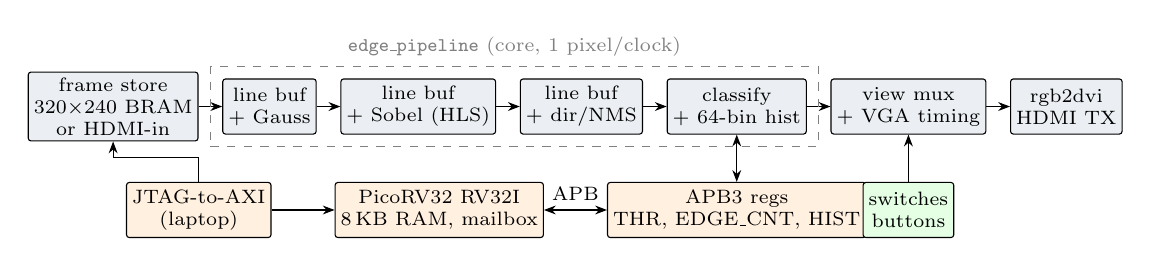
\begin{tikzpicture}[font=\scriptsize, node distance=3mm, blk/.style={draw, rounded corners=1pt, fill=iitblue!8, minimum height=7mm, align=center, inner sep=2pt}, >={Stealth[length=1.5mm]}]
\node[blk] (src) {frame store\\320$\times$240 BRAM\\or HDMI-in};
\node[blk, right=of src] (lb1) {line buf\\+ Gauss};
\node[blk, right=of lb1] (lb2) {line buf\\+ Sobel (HLS)};
\node[blk, right=of lb2] (lb3) {line buf\\+ dir/NMS};
\node[blk, right=of lb3] (cls) {classify\\+ 64-bin hist};
\node[blk, right=of cls] (vid) {view mux\\+ VGA timing};
\node[blk, right=of vid] (tx) {rgb2dvi\\HDMI TX};
\foreach \a/\b in {src/lb1,lb1/lb2,lb2/lb3,lb3/cls,cls/vid,vid/tx} \draw[->] (\a) -- (\b);
\node[blk, below=6mm of cls, fill=orange!12] (apb) {APB3 regs\\THR, EDGE\_CNT, HIST};
\node[blk, left=8mm of apb, fill=orange!12] (cpu) {PicoRV32 RV32I\\8\,KB RAM, mailbox};
\node[blk, left=8mm of cpu, fill=orange!12] (jtag) {JTAG-to-AXI\\(laptop)};
\node[blk, below=6mm of vid, fill=green!10] (sw) {switches\\buttons};
\draw[<->] (cpu) -- node[above]{APB} (apb); \draw[<->] (apb) -- (cls);
\draw[->] (jtag) -- (cpu); \draw[->] (jtag.north) |- ($(src.south)+(0,-2mm)$) -- (src.south);
\draw[->] (sw) -- (vid);
\node[draw, dashed, gray, fit=(lb1)(cls), inner sep=1.5mm, label={[gray]above:\texttt{edge\_pipeline} (core, 1 pixel/clock)}] {};
\end{tikzpicture}
\caption{Top-level block diagram (board top \texttt{zybo\_hdmi\_top}). The dashed box is the core reported in Sections 4--8.}\label{fig:block}
\end{figure}

\begin{table}[H]\centering\footnotesize
\caption{APB3 register map (\texttt{rtl/apb\_regs.sv}, base 0x1000\_0000 for the RV32 core; PREADY=1, PSLVERR on unmapped or read-only writes).}\label{tab:regmap}
\setlength{\tabcolsep}{3pt}\begin{tabular}{@{}lllp{9.0cm}@{}}
\toprule
Offset & Name & Acc. & Description\\
\midrule
0x00 & CTRL & RW & bit0 enable, 1 auto\_threshold, 3:2 view, 4 hyst, 5 threshold\_cpu (CPU owns thresholds), bit6 W: clear histogram\\
0x04/0x08 & THR\_HI/THR\_LO & RW & 11-bit thresholds (reset 200/80), applied at the next frame\\
0x0C & STATUS & RW1C & sticky: frame\_done, fifo under/overflow, sync\_error, hist\_valid, crc\_match (set wins over clear)\\
0x10/0x14 & EDGE\_CNT/FRAME\_CNT & RO & strong-edge pixels of the last frame; frame counter\\
0x20/0x24 & THR\_*\_AUTO & RO & reserved for the adaptive unit (reads 0 in the board build)\\
0x2C/0x30 & HIST\_IDX/HIST\_DATA & RW/RO & select one of 64 histogram bins (bin = NMS[10:5]); read its 19-bit count\\
0x34 & VERSION & RO & 0x5037\_0300\\
\bottomrule
\end{tabular}
\end{table}
\textbf{Golden model.} \texttt{model/golden.py} (NumPy) implements every stage with the exact integer arithmetic above and
writes hex vectors of all intermediate stages (gray, smooth, magnitude, direction, NMS, class, histogram) for the
testbenches. A second, independent implementation written by the second team member agrees on all 70 stage arrays of
10 images, so a misreading of the specification by one of us would have shown up as a disagreement. Figure~\ref{fig:stages} shows the stages on one image.
\textbf{Y-chart.} The design was specified in the behavioural domain (algorithm, golden model), refined to the structural
RTL domain (datapath + FSMs, hand HLS), and mapped to the physical domain by Vivado on the xc7z010.
\figfile{stages.png}{0.78\linewidth}{Golden-model stages on the 640$\times$480 \emph{camera} image (the RTL output is identical bit for bit).}{fig:stages}

%% =====================================================================
\section{High-Level Representation and Hand HLS}
\label{sec:hls}
\subsection{CDFG and Transformations}
The kernel is the Sobel window operator: from the 3$\times$3 smoothed window $p_{rc}$ compute $G_x$, $G_y$, $|G_x|$,
$|G_y|$, the magnitude and the two direction comparators. Starting from the textbook 3$\times$3 convolution (loop over
nine taps per gradient) we applied four transformations~\cite{demicheli} (Table~\ref{tab:transform}); counts and critical paths are computed by
\texttt{hls/sobel\_hls.py} from the DFG of each version (one control step per add/sub/compare/abs/multiply, shifts are wiring).
\textbf{Constant folding / dead-code elimination} removes the six zero taps and the $\times(\pm1)$ products;
\textbf{strength reduction} (hardware-library transformation) turns $\times2$, $\times32$ into wiring and $\times13$ into
$(x\ll3)+(x\ll2)+x$; \textbf{tree-height reduction} rewrites $G_x=((p_{02}-p_{00})+(p_{22}-p_{20}))+2(p_{12}-p_{10})$;
\textbf{CSE} shares $E_1=p_{22}-p_{00}$ and $E_2=p_{02}-p_{20}$, since $G_x=E_1+E_2+2F$ and $G_y=E_1-E_2+2G$ with
$F=p_{12}-p_{10}$, $G=p_{21}-p_{01}$.

\begin{table}[H]\centering\footnotesize
\caption{Effect of the transformations on the Sobel kernel (from the DFGs).}\label{tab:transform}
\begin{tabular}{@{}lcccc@{}}
\toprule
Version & \#Mult & \#Add/Sub/Cmp & \#Abs & Crit.\ path\\
\midrule
Original 3$\times$3 convolution (loop order) & 22 & 19 & 2 & 12\\
+ constant folding, dead-code elimination & 8 & 13 & 2 & 9\\
+ strength reduction ($\times13$ shift-add) & 0 & 17 & 2 & 9\\
+ tree-height reduction & 0 & 17 & 2 & 7\\
+ CSE of $E_1$, $E_2$ (shipped kernel, Fig.~\ref{fig:cdfg}) & 0 & 15 & 2 & 7\\
\bottomrule
\end{tabular}
\end{table}
\figfile{cdfg.pdf}{0.95\linewidth}{Data-flow graph of the final kernel (blue: add/sub/compare, yellow: absolute value).}{fig:cdfg}

\subsection{Operator Library}
Each operator was characterised register-to-register on the xc7z010-1 by Vivado place-and-route (\texttt{hls/oplib.sv}):
9-bit subtract 8 LUT / 1.90\,ns, 11-bit add 11 LUT / 2.26\,ns, 11-bit abs 12 LUT / 1.85\,ns, $\times13$ shift-add 20 LUT / 2.51\,ns,
16-bit compare 8 LUT / 2.31\,ns, 16-bit shared add/sub/compare ALU 24 LUT / 2.40\,ns, 16-bit abs 31 LUT / 2.74\,ns (path includes
clock-to-out and setup). The chained magnitude + $\times13$ + compare used in one pipeline stage takes 4.21\,ns. At the 39.7\,ns pixel
clock several operators can be chained per cycle, which the shipped 4-stage schedule exploits; the scheduling below uses
the strict one-operation-per-step model of the course.

\subsection{Scheduling}
With latency bound $\lambda=7$ (the critical path), ASAP/ALAP give mobility 0 for 14 of the 17 operations; only $F$, $G$
(mobility 1) and the magnitude add (mobility 2) can move (Table~\ref{tab:asap}). ASAP needs 4 adders and 2 abs units in step 1/4.
List scheduling with priority = longest path to a sink (ties: lower mobility) gives \textbf{9 steps} with 2 adders + 1 abs unit,
and \textbf{15 steps} with 1 adder + 1 abs unit. An exact time-constrained ILP (\texttt{scipy.optimize.milp}, binary $x_{i,t}$,
precedence and per-step resource constraints) gives the minimum units for each latency: $\lambda=7$: 3 adders + 2 abs;
$\lambda=8$: 3 + 1; $\lambda=9$--14: 2 + 1; $\lambda\ge15$: 1 + 1. Both list schedules are therefore optimal for their resources.

\begin{table}[H]\centering\scriptsize
\caption{ASAP, ALAP ($\lambda=7$), mobility, and the list schedule with 2 adders + 1 abs unit.}\label{tab:asap}
\setlength{\tabcolsep}{3pt}
\begin{tabular}{@{}lccccccccccccccccc@{}}
\toprule
Op & $E_1$ & $E_2$ & $F$ & $G$ & $P$ & $Q$ & $G_x$ & $G_y$ & $|G_x|$ & $|G_y|$ & mag & $8a{+}4a$ & $13|G_x|$ & $8b{+}4b$ & $13|G_y|$ & $c_0$ & $c_2$\\
\midrule
ASAP & 1&1&1&1&2&2&3&3&4&4&5&5&6&5&6&7&7\\
ALAP & 1&1&2&2&2&2&3&3&4&4&7&5&6&5&6&7&7\\
Mobility & 0&0&1&1&0&0&0&0&0&0&2&0&0&0&0&0&0\\
List (2A+1B) & 1&1&3&3&2&2&4&4&5&6&9&6&7&7&8&8&9\\
\bottomrule
\end{tabular}
\end{table}

\subsection{Allocation and Binding}
\textbf{Register binding (left-edge~\cite{demicheli}).} Lifetimes of the 15 values of the 9-step schedule, sorted by birth step, pack into
4 registers: R0=$\{E_1,P,G_x,|G_x|,\text{mag}\}$, R1=$\{E_2,Q,G_y,8a{+}4a,13|G_x|,13|G_y|\}$, R2=$\{F,|G_y|\}$, R3=$\{G,8b{+}4b\}$
(the 1-bit comparator results and signs go to flag flip-flops). This equals the maximum number of simultaneously live
values, so left-edge is optimal here (the lifetimes form an interval graph).
\textbf{FU binding (clique partitioning).} In the compatibility graph of the 15 add-type operations two operations are
compatible if they are in different control steps (Fig.~\ref{fig:compat}). The greedy clique partitioning (merge the pair with
the most common neighbours) yields two cliques, ADD0=$\{E_1,P,F,G_x,8a{+}4a,13|G_x|,c_0,\text{mag}\}$ and
ADD1=$\{E_2,Q,G,G_y,8b{+}4b,13|G_y|,c_2\}$, and one abs unit for $\{|G_x|,|G_y|\}$.
\figfile{compat.pdf}{0.30\linewidth}{Compatibility graph of the add-type operations for the 9-step schedule; colours are the two cliques (= two adders); labels give the control step.}{fig:compat}

\subsection{FSMD and Design Points}
The script turns a schedule and binding into an FSMD (\texttt{rtl/study/sobel\_fsmd\_*.sv}): a step counter is the controller;
each state drives the operand multiplexers and the operation (add/sub/compare) of each unit and the enables of the bound
registers. Both FSMDs equal the shipped pipelined \texttt{sobel.sv} on 100{,}000 windows (random, extreme 0/255 and impulses).
Table~\ref{tab:designpoints} compares them with the shipped II$=$1 pipeline (Vivado OOC, 4\,ns target).

\begin{table}[H]\centering\footnotesize
\caption{Design points on the xc7z010-1 (place and route, out of context).}\label{tab:designpoints}
\begin{tabular}{@{}lcccccc@{}}
\toprule
Design point & LUT & FF & DSP & F$_\text{max}$ & Latency & Throughput\\
\midrule
Pipelined II$=$1, 4 chained stages (shipped) & 141 & 97 & 0 & 192\,MHz & 4 clk & 1 window/clk\\
FSMD 2 adders + 1 abs & 358 & 143 & 0 & 181\,MHz & 9+1 clk & 1 per 10 clk\\
FSMD 1 adder + 1 abs (min.\ operators) & 256 & 139 & 0 & 186\,MHz & 15+1 clk & 1 per 16 clk\\
\bottomrule
\end{tabular}
\end{table}
The design point with the fewest operators is \emph{not} the smallest on the FPGA: a shared unit must be as wide as its widest
operation (16 bits for the comparators, against 9--11 bits for most operations in the pipeline), and every shared input
needs a multiplexer that costs as much as the 2-LUT-per-bit adder it saves. Resource sharing pays only when the shared
operator is expensive (multipliers, DSPs). Because the video needs one window per clock, only the pipelined point meets
the specification, and it is the one we used.

%% =====================================================================
\section{Logic and FSM Optimisation}
\label{sec:logic}
The control FSM studied here is the controller of the adaptive-threshold unit (\texttt{rtl/otsu\_ctrl.sv},
Section~\ref{sec:paper}). Its inputs are \emph{en, sof, eof} (frame start/end), \emph{odone} (Otsu sweep done), \emph{cdone} (clear pass
done), \emph{px} (a pixel of the next frame has arrived) and \emph{ovr} (overrun); its Mealy outputs control counting,
clearing, bank swap and threshold update.
\subsection{State Minimisation}
The STG written from the specification had 7 states: INIT (after reset), RECOVER (after an overrun or disable), ARM,
COLLECT, SWEEP, CLEAR, PEND. The implication chart (\texttt{logic/logic\_study.py}, all $2^7$ input combinations per pair)
marked 20 of the 21 pairs as distinguishable by outputs in the first pass; the only remaining pair, (INIT, RECOVER), has
identical outputs and only the implied pair (INIT, RECOVER) itself, so it is never marked: INIT $\equiv$ RECOVER. Merging them
gives the 6-state machine of Fig.~\ref{fig:stg}; a second chart on it finds no equivalent pair, so it is minimal.
\begin{figure}[H]\centering
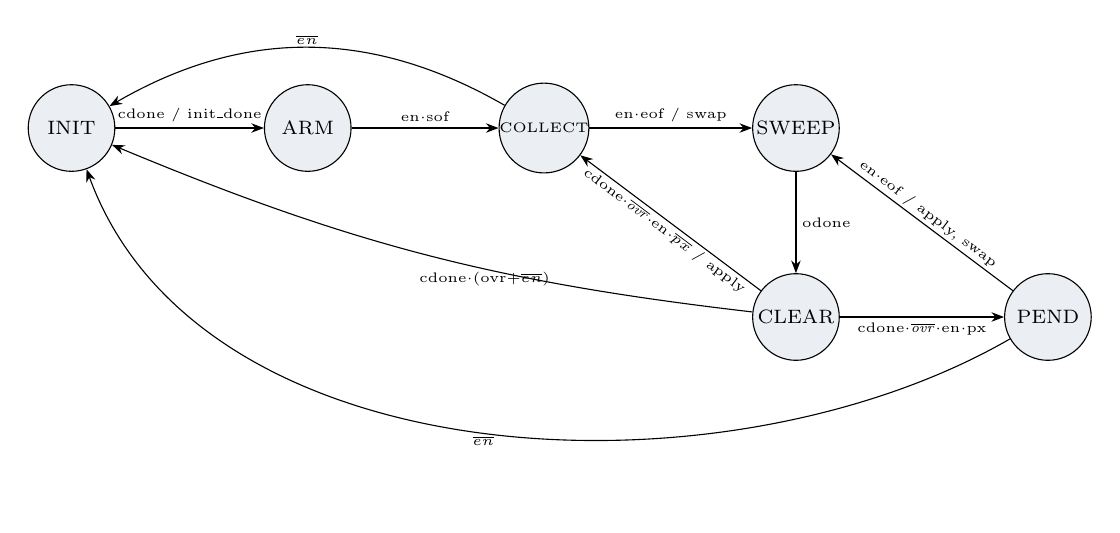
\begin{tikzpicture}[font=\scriptsize, >={Stealth[length=1.6mm]}, st/.style={draw, circle, minimum size=11mm, inner sep=0pt, fill=iitblue!8}, lab/.style={font=\tiny, inner sep=1pt}]
\node[st] (I) at (0,0) {INIT}; \node[st] (A) at (3.0,0) {ARM}; \node[st] (C) at (6.0,0) {\tiny COLLECT};
\node[st] (S) at (9.2,0) {SWEEP}; \node[st] (L) at (9.2,-2.4) {CLEAR}; \node[st] (P) at (12.4,-2.4) {PEND};
\draw[->] (I) -- node[lab, above=1pt]{cdone / init\_done} (A);
\draw[->] (A) -- node[lab, above=1pt]{en$\cdot$sof} (C);
\draw[->] (C) -- node[lab, above=1pt]{en$\cdot$eof / swap} (S);
\draw[->] (S) -- node[lab, right=1pt]{odone} (L);
\draw[->] (L) -- node[lab, below=1pt]{cdone$\cdot\overline{\mathit{ovr}}\cdot$en$\cdot$px} (P);
\draw[->] (L) -- node[lab, sloped, below, pos=0.5]{cdone$\cdot\overline{\mathit{ovr}}\cdot$en$\cdot\overline{px}$ / apply} (C);
\draw[->] (P) -- node[lab, sloped, above, pos=0.5]{en$\cdot$eof / apply, swap} (S);
\draw[->] (C) to[bend right=30] node[lab, above]{$\overline{en}$} (I);
\draw[->] (L) to[bend left=8] node[lab, below, pos=0.4]{cdone$\cdot$(ovr$+\overline{en}$)} (I);
\draw[->] (P) to[out=-150, in=-70, looseness=0.9] node[lab, below]{$\overline{en}$} (I);
\end{tikzpicture}
\caption{Minimised controller STG (self-loops, taken when no labelled condition holds, are omitted).}\label{fig:stg}
\end{figure}
\subsection{State Encoding}
Besides Vivado's encodings we applied the lecture's adjacency heuristic: weight $w_{ij}$ = 2 if $s_i,s_j$ share a successor under
some input, +1 per common predecessor, +1 for equal outputs, +1 if adjacent; an exhaustive search over 3-bit codes minimised
$\sum w_{ij}\,d_H(c_i,c_j)$ (cost 57 against 72 for plain binary) and gave INIT=000, ARM=001, COLLECT=011, PEND=010,
SWEEP=110, CLEAR=111. All encodings were synthesised with registered inputs/outputs (Vivado log confirms each re-encoding;
the user codes use \texttt{-fsm\_extraction off}).
\begin{table}[H]\centering\footnotesize
\caption{State encoding comparison for \texttt{otsu\_ctrl} (FF includes 14 I/O registers of the wrapper).}\label{tab:encoding}
\begin{tabular}{@{}lcccc@{}}
\toprule
Encoding & State bits & LUT & FF & F$_\text{max}$ (MHz)\\
\midrule
Binary (declaration order, extraction off) & 3 & 16 & 17 & 424\\
Sequential (Vivado) & 3 & 16 & 17 & 406\\
Gray (Vivado) & 3 & 17 & 17 & 445\\
Johnson (Vivado) & 3 & 16 & 17 & 445\\
One-hot (Vivado) & 6 & \textbf{12} & 20 & 408\\
Heuristic adjacency (ours, extraction off) & 3 & 15 & 17 & 417\\
\bottomrule
\end{tabular}
\end{table}
One-hot needs the fewest LUTs (each next-state bit depends on few state bits, which suits 6-input LUTs) at the cost of 3 extra
flip-flops; the heuristic code beats plain binary by one LUT. For a controller this small all encodings are far above the 25\,MHz
requirement, so the choice is not critical.

\subsection{Two-Level Minimisation}
The ESPRESSO~\cite{espresso}/BDD block is the direction quantiser + NMS select. Its inputs are the two comparator bits $c_0$
($32|G_y|\le13|G_x|$), $c_2$, the gradient signs $s_x,s_y$ and the eight neighbour comparisons ($m\ge$ earlier, $m>$ later
for each sector); $c_0c_2(s_x+s_y)$ cannot occur and is a don't-care. Results (Table~\ref{tab:twolevel}):
\begin{table}[H]\centering\footnotesize
\caption{Two-level minimisation. Our QM/UCP, ESPRESSO heuristic and ESPRESSO \texttt{-Dexact} reach the same cost.}\label{tab:twolevel}
\setlength{\tabcolsep}{3pt}\begin{tabular}{@{}lccccc@{}}
\toprule
Function (inputs) & On / DC minterms & Canonical (terms/lit.) & Primes & QM+UCP & ESPRESSO heur./exact\\
\midrule
dir[1] (4) & 6 / 3 & 6 / 24 & 5 & 3 / 8 & 3 / 8 \;\; 3 / 8\\
dir[0] (4) & 4 / 3 & 4 / 16 & 3 & 1 / 2 & 1 / 2 \;\; 1 / 2\\
NMS keep (12) & 832 / 768 & 832 / 9984 & 27 & 6 / 31 & 6 / 31 \;\; 6 / 31\\
\bottomrule
\end{tabular}
\end{table}
Our tabular QM merged 1600 cubes through 9 columns into 27 primes for \emph{keep}; the unate covering problem (832 rows $\times$ 27
columns) was solved completely by essential columns (6 essential primes) and row/column dominance, so the cyclic core was empty and
branch-and-bound needed a single node. The generated \texttt{rtl/dir\_decide.sv} is
$\mathit{dir}[1]=\bar c_0\bar s_x s_y+\bar c_0 s_x\bar s_y+\bar c_0c_2$, $\mathit{dir}[0]=\bar c_0\bar c_2$ (4 terms/10 literals instead of 10/40).

\subsection{Multilevel Optimisation}
Algebraic kernel extraction on the 6-cube \emph{keep} cover found 9 kernels, e.g.\ co-kernel $\bar c_0\bar c_2\,ge_{NE}gt_{SW}$ with
kernel $s_x\bar s_y+\bar s_xs_y$ (an XOR) and co-kernel $\bar c_0\bar c_2$ with the four-cube diagonal kernel. Extracting them gives
$\mathit{keep}=c_0\,ge_Wgt_E+\bar c_0c_2\,ge_Ngt_S+\bar c_0\bar c_2[(s_x\odot s_y)ge_{NW}gt_{SE}+(s_x\oplus s_y)ge_{NE}gt_{SW}]$ with
17 literals (an XOR counted as two) against 31 in the minimum SOP, i.e.\ exactly the ``sector decode, then select'' structure of the RTL.
Yosys+ABC on the RTL gives 19 AND + 20 NOT (AIG), 8 gates with XOR/MUX (4 AND, 3 MUX, 1 XNOR), 5 LUT4 or 3 LUT6:
the multiplexer-based factored form is what both our kernels and ABC arrive at.

%% =====================================================================
\section{RTL Design and SoC Integration}
\label{sec:rtl}
\subsection{Module Hierarchy}
\texttt{edge\_pipeline} (core) = \texttt{linebuf}$\times$3 + \texttt{gauss} + \texttt{sobel} (with \texttt{dir\_decide}) +
\texttt{dirnms} + \texttt{classify\_hist}. \textbf{Line buffer:} two 640-entry BRAM rows used alternately (the row being
overwritten holds line $y-2$), synchronous read-first, plus a 3$\times$3 register window; a window is valid only when its centre is
at least one pixel inside the frame, and coordinates are carried with the data, so the pipeline tolerates any gaps in
\texttt{valid}. \textbf{Gauss:} one registered stage, shift-add only. \textbf{Sobel:} the 4-stage chained schedule of the hand HLS
(stage 0: $E_1,E_2,F,G$; 1: $G_x,G_y$; 2: abs and signs; 3: magnitude, comparators, \texttt{dir\_decide}). \textbf{NMS:}
combinational select of the earlier/later neighbour on a 13-bit (direction+magnitude) window. \textbf{Classifier:} one
registered stage plus a 64-bin histogram of non-zero NMS values in two banks that swap at the end of each frame (the
finished bank is the readable snapshot). Single clock, synchronous active-high reset, valid/SOF/EOL handshake with no back
pressure (the video source never stalls). The latency from a pixel entering the core to its class is 3 lines + 15 clocks
(2{,}415 clocks at an 800-clock line, measured by \texttt{tb\_latency.sv}); the board delays the original and smoothed views by
the same amount so that all four views stay aligned. \texttt{verilator --lint-only -Wall} on the core reports only 11
\texttt{UNUSEDSIGNAL} warnings (unused rounding bits and the direction bits of NMS neighbours, intentional) and one file-name
warning; the new controller is lint-clean.
\textbf{Board top} (\texttt{zybo\_hdmi\_top}): MMCM 25.18/125.9\,MHz, \texttt{vga\_timing} (800$\times$525 counters), stored-image
source (320$\times$240$\times$8-bit BRAM frame store, shown 2$\times$), view mux (SW1:0 original/smoothed/strong/classes), threshold
presets (SW3:2), Digilent \texttt{rgb2dvi}. In the \emph{live} build an HDMI receiver (Digilent \texttt{dvi2rgb}) takes the laptop's
800$\times$600 webcam picture, converts to gray, downsamples 2.5:1 to 320$\times$240 and writes it through an asynchronous FIFO
into the same frame store, which is read on the 25.18\,MHz output clock.

\subsection{Bus Integration, Interrupt and DMA}
The PicoRV32~\cite{picorv32} subsystem (\texttt{rtl/soc}) has 8\,KB RAM, a mailbox shared with the laptop, a GPIO word and an APB3 master (SETUP
$\rightarrow$ ACCESS) to \texttt{apb\_regs}. The laptop loads firmware and photos through JTAG-to-AXI. Once per frame the firmware
reads EDGE\_CNT and all 64 bins and writes the next thresholds (Listing~\ref{lst:driver}). There is \textbf{no interrupt}: the
firmware polls FRAME\_CNT, which is enough at 60 frames/s. There is \textbf{no DMA}: a DDR frame buffer would need the Zynq PS and an
AXI VDMA; the BRAM frame store written over JTAG (or by the HDMI receiver) is our memory-to-video path.
\begin{lstlisting}[language=C,caption={Driver excerpt (\texttt{fw/src/main.c}).},label={lst:driver}]
#define APB(off) (*(volatile u32 *)(0x10000000u + (off)))
APB(CTRL) = 0x21;                              // enable, thresholds owned by the CPU
for (;;) { u32 f = APB(FRAME_CNT); if (f == last) continue; last = f;
  u32 edges = APB(EDGE_CNT);
  for (u32 i = 0; i < 64; i++) { APB(HIST_IDX) = i; hist[i] = APB(HIST_DATA); }
  APB(CTRL) = 0x21; APB(THR_LO) = nlo; APB(THR_HI) = nhi; }  // CTRL re-asserted: BTN0 resets the bank
\end{lstlisting}

\subsection{Hardware/Software Comparison}
The whole pipeline was also written in C (\texttt{fw/swedge/swedge.c}, bit-exact with the golden model) and run on the
\emph{same} PicoRV32 configuration (RV32I, no multiplier, no barrel shifter, one memory wait state) in simulation
(\texttt{tb/soc/tb\_swedge.sv}); all 768 classes of a 32$\times$24 image match the model. It takes 335{,}563 cycles with
\texttt{-O2} (437 cycles/pixel; 486 with \texttt{-Os}). The hardware core takes one cycle per pixel plus a 3-line fill, so the
speed-up is about \textbf{437$\times$}. At 640$\times$480 the software would need 134 million cycles, 5.3\,s per frame at 25\,MHz
(0.19 frame/s), against 60 frames/s in hardware. This is why the CPU only supervises (reads statistics, sets thresholds) and the
pixel work is in hardware: the per-frame firmware loop takes a few thousand cycles out of 420{,}000.

%% =====================================================================
\section{Simulation-Based Verification}
\label{sec:sim}
\textbf{Testbench architecture.} Self-checking testbenches read the golden-model vectors and compare \emph{every stage}
(smooth, magnitude, direction, NMS, class, coordinates, SOF/EOL markers, histogram bins) at the expected raster position, so a
missing, duplicated or shifted pixel is detected, not only a wrong value. Three stimulus modes: continuous, random gaps, and
VESA blanking. Directed tests: black/white frames, checkerboard, ramps, steps, diagonals, threshold corner cases (0/0, 1/1,
equal, 2047); random: 25 random frames per small size; natural: 10 corpus images and a photo at 640$\times$480.
Unit/stress benches: Sobel extrema and 100{,}000 random windows, an \textbf{exhaustive 4{,}169{,}764-case} direction test, NMS ties,
histogram saturation, line-buffer restart, APB, CRC. System benches: the full video path (28 runs over the 4 views and 4 presets), the
RV32 SoC with real firmware (6 scenarios) and the live HDMI-in path (all 76{,}800 frame-store bytes).

\textbf{Assertions.} Following the assertion-based style of~\cite{bening}, 13 concurrent SVA assertions are attached with \texttt{bind} (\texttt{tb/sva/core\_sva.sv}, the RTL is
unchanged) and run in Verilator with \texttt{--assert} during the regression: windows centred inside the image (A1), line pointers
in range (A2), EOL wraps the column (A3), $|G_x|+|G_y|\le2040$ (A4), Sobel latency exactly 4 with II$=$1 (A5,
Listing~\ref{lst:sva}), class never 2'b11 (A6), one class per NMS pixel one clock later (A7), strong implies $m\ge T_\text{hi}$
(A8), frame end swaps histogram banks (A9), output coordinates within $[3,W{-}4]\times[3,H{-}4]$ (A10), SOF/EOL markers (A11, A12),
NMS never invents a magnitude (A13); 4 cover properties (weak class, strong class, diagonal direction, end of frame) are all hit
(31$\times$23 regression, 42 frames, 3 timing modes). A mutant
classifier that outputs 2'b11 fails A6.
\begin{lstlisting}[language=Verilog,caption={Assertion A5: initiation interval 1 and fixed latency of the hand-HLS Sobel.},label={lst:sva}]
a_latency4: assert property (@(posedge clk) out_valid == $past(in_valid, 4));  // in module sobel_sva
bind sobel sobel_sva u_sva (.*);                                                 // attached without editing the RTL
\end{lstlisting}
\begin{table}[H]\centering\footnotesize
\caption{Verification summary.}\label{tab:simsummary}
\begin{tabularx}{\linewidth}{@{}Xr@{}}
\toprule
Item & Result\\
\midrule
Core regressions (6 sizes 7$\times$7 \ldots 640$\times$480, 3 timing modes) & 18/18 PASS\\
Pixels compared bit-exactly with the model at 640$\times$480 (33 frames $\times$ 3 modes), 0 mismatches & 29{,}751{,}084\\
Unit + stress benches; video (28 runs); SoC (6 scenarios); HDMI-in & all PASS\\
Exhaustive direction cases / random Sobel windows (0 mismatches) & 4{,}169{,}764 / 100{,}000\\
Assertions (concurrent SVA) / cover properties (31$\times$23 run) & 13 (0 failures) / 4 (all hit)\\
Line + toggle coverage of the core RTL (Verilator; 4 modules at 100\%, classifier 87.7\%) & 96.3\%\\
RTL mutants caught by the scoreboard & 7/7\\
\bottomrule
\end{tabularx}
\end{table}
The uncovered points are the histogram saturation branches (a 19-bit counter cannot saturate in a 31$\times$23 frame; they are
tested separately by \texttt{tb\_hist\_stress}) and toggles of the upper coordinate bits at this small size.
\textbf{Bugs found by simulation:} a zero NMS value became ``weak'' when $T_\text{lo}=0$ (now always class 0); a histogram clear
dropped the class of the pixel in the same cycle; an APB status event was lost when software cleared it in the same cycle
(now set-dominant, later proved in SymbiYosys). On hardware: BTN0 reset the
APB bank and silently returned thresholds to the switch presets (firmware now re-asserts CTRL every frame).

%% =====================================================================
\section{Formal Verification}
\label{sec:formal}
\subsection{Kripke Structure and CTL Labelling}
The controller of Fig.~\ref{fig:stg} is abstracted to a Kripke structure $M=(S,R,L)$ with $S=\{$INIT, ARM, COLLECT, SWEEP,
CLEAR, PEND$\}$, $R$ = the STG edges plus self-loops (inputs are existentially abstracted), and atomic propositions
$\mathit{collect}$ (counting), $\mathit{sweep}$, $\mathit{clear}$, $\mathit{pend}$. \textbf{(a) $\mathbf{EF}\,\mathit{pend}$}
(backward reachability): label PEND; its predecessors CLEAR; then SWEEP; then COLLECT and PEND; then ARM; then INIT. Every state is
labelled, so the property holds in the initial state. \textbf{(b) $\mathbf{EG}\,\neg\mathit{clear}$} (SCC algorithm): restricting $M$ to
$\neg\mathit{clear}$ states leaves $\{$INIT, ARM, COLLECT, SWEEP, PEND$\}$; each has a self-loop, so each is a non-trivial SCC and
all five are labelled. In particular SWEEP satisfies $\mathbf{EG}\neg\mathit{clear}$: a path can stay in SWEEP forever if the Otsu
unit never answers. This is why the liveness property P8 below fails without fairness and needs \texttt{FAIRNESS odone}; with the
fair-EG algorithm, the SWEEP self-loop is not a fair SCC and the label disappears. Both hand results agree with NuSMV.

\subsection{Model Checking with NuSMV}
The RTL is exported with Yosys \texttt{write\_smv}; free inputs become unconstrained variables, reset is the initial state.
Table~\ref{tab:ctl} lists the 12 controller properties (\texttt{formal/otsu\_ctl.py}); NuSMV also confirms that the transition
relation is total (no deadlock state). Fairness assumptions describe a working environment: the sweep and the clear pass eventually
finish, frames keep ending, and some frame starts while enabled. In addition the shipped raster generator \texttt{vga\_timing}
satisfies 10 CTL properties on frame/line synchronisation (counter bounds, SOF only at the origin, EOL only in active video, line
and frame wrap, $\mathbf{AG\,EF}\,\mathit{sof}$, $\mathbf{AG\,EF}\,\mathit{eof}$, EOF$\Rightarrow$EOL, no deadlock) and the stream checker
\texttt{ctrl\_sync} 3 more; 5+3 RTL mutants of those two modules are each caught (Appendix~\ref{app:ctl}).
\begin{table}[H]\centering\footnotesize
\caption{CTL properties of the controller RTL checked with NuSMV 2.6 (s = \texttt{state}).}\label{tab:ctl}
\setlength{\tabcolsep}{4pt}
\begin{tabularx}{\linewidth}{@{}clXc@{}}
\toprule
\# & Type & CTL formula & Result\\
\midrule
1 & Safety & $\mathbf{AG}\,\neg(\mathit{clr\_both}\wedge\mathit{count\_en})$ & true\\
2 & Safety & $\mathbf{AG}\,\neg(\mathit{clr\_both}\wedge\mathit{clr\_one})$ & true\\
3 & Safety (frame-aligned update) & $\mathbf{AG}(\mathit{apply}\rightarrow(s{=}\text{PEND}\wedge\mathit{eof})\vee(s{=}\text{CLEAR}\wedge\neg\mathit{px}))$ & true\\
4 & Safety & $\mathbf{AG}(\mathit{swap}\rightarrow\mathbf{AX}\,s{=}\text{SWEEP})$ & true\\
5 & Safety & $\mathbf{AG}(s\le 5)$ (legal codes only) & true\\
6 & Reachability & $\mathbf{EF}(s{=}\text{PEND}\wedge\mathit{apply})$ & true\\
7 & Non-blocking & $\mathbf{AG\,EF}\,s{=}\text{INIT}$ & true\\
8 & Liveness & $\mathbf{AG}(s{=}\text{SWEEP}\rightarrow\mathbf{AF}\,s{=}\text{CLEAR})$ & \textbf{false}\\
9 & Liveness (fair) & same as 8 under the fairness constraints & true\\
10 & Liveness (fair) & $\mathbf{AG}(\mathit{swap}\rightarrow\mathbf{AX\,AF}(\mathit{apply}\vee s{=}\text{INIT}))$ & true\\
11 & Until (fair) & $\mathbf{AG}(s{=}\text{SWEEP}\rightarrow\mathbf{A}[\mathit{count\_en}\;\mathbf{U}\;s{=}\text{CLEAR}])$ & true\\
12 & Liveness (fair) & $\mathbf{AG\,AF}(s{=}\text{COLLECT}\vee s{=}\text{PEND})$ & true\\
\bottomrule
\end{tabularx}
\end{table}
Property 8 is false for the reason found by hand in (b). A first version of property 12, $\mathbf{AG\,AF}\,s{=}\text{COLLECT}$, was
false even with fairness: with no blanking the controller legitimately cycles PEND$\rightarrow$SWEEP$\rightarrow$CLEAR$\rightarrow$PEND,
so the specification was corrected rather than the RTL.

\subsection{Bug Injection and Counterexamples}
\textbf{B1:} CLEAR applies the new threshold even when a pixel of the next frame has already arrived (the PEND branch removed).
P3 and P6 fail; the counterexample is INIT $\xrightarrow{cdone}$ ARM $\xrightarrow{en,sof}$ COLLECT $\xrightarrow{en,eof}$ SWEEP
$\xrightarrow{odone}$ CLEAR $\xrightarrow{en,cdone,px}$ \emph{apply}. Replayed in simulation with the same conditions (a stream without
blanking, so \emph{px} is set when the clear ends) the full enhanced pipeline reports ``thresholds changed inside frame 1 at
(5,5)''. \textbf{B2:} CLEAR also waits for \emph{odone}, which only pulses in SWEEP. P10 and P12 fail with a lasso counterexample
that loops in CLEAR; replayed with blanking, the adaptive threshold is never applied and the class map differs from the paper
engine's (``CLASS MISMATCH (24,4)'').

\subsection{BDD Analysis}
With the \texttt{dd} ROBDD~\cite{bryant} package (\texttt{formal/bdd\_study.py}) we built the direction comparator $c_0=(32|G_y|\le13|G_x|)$
bit by bit on the real 11-bit operands (22 variables, ripple-carry adders and a comparator).
\begin{table}[H]\centering\footnotesize
\caption{ROBDD node counts for the comparator $c_0$ (22 variables).}\label{tab:bdd}
\begin{tabular}{@{}lc@{}}
\toprule
Variable ordering & Nodes\\
\midrule
Interleaved, MSB first ($a_{10},b_{10},a_9,b_9,\ldots$) & 554\\
Interleaved, LSB first & 403\\
Blocked (all $|G_x|$ bits, then all $|G_y|$ bits) & 4{,}085\\
Blocked, after Rudell sifting~\cite{rudell} (fixed seed; 228--405 over six seeds) & \textbf{283}\\
\bottomrule
\end{tabular}
\end{table}
The blocked order must remember all of $|G_x|$ before it sees $|G_y|$, hence the 10$\times$ blow-up. Sifting is greedy and its result
depends on the order in which variables are visited, but every run ended far below the blocked order and usually below both interleavings. For NMS-select, ordering the sector bits first gives 14--17 nodes against 43--53 with the comparator bits first.
\textbf{Equivalence:} the specification (on the care set), our QM/UCP cover, the ESPRESSO cover and the RTL after Yosys+ABC mapping
(read back from BLIF) all reduce to the same ROBDD node, so they are equivalent. \textbf{Symbolic reachability} of the controller
RTL (next-state functions from Yosys, image computation by existential quantification) reaches a fixed point after 6 iterations with
6 of the 8 codes reachable, matching NuSMV's count of 6 reachable states.

\subsection{Formal Verification of the RTL (SymbiYosys)}
SymbiYosys (smtbmc, z3) proved three harnesses (\texttt{formal/sby}) both by BMC to depth 30 and \textbf{unboundedly by k-induction}
(depth 20): \texttt{vga\_timing} at the \emph{real} 800$\times$525 parameters (8 assertions: counter bounds, SOF/EOL/EOF/DE
placement, HSYNC position, line wrap), so the real size is covered and not only the reduced NuSMV model; \texttt{otsu\_ctrl} (7 assertions, incl.
frame-aligned update and ``CLEAR holds until the pass ends''); \texttt{apb\_regs} (6 assertions: PREADY, PSLVERR only in ACCESS,
read-only registers reject writes, no spurious writes, a status event is never lost, a write lands).

%% =====================================================================
\section{Incorporating the Research Paper}
\label{sec:paper}
\textbf{First attempt.} The paper's engine (frame buffer, 256-bin histogram, log-domain Otsu, classifier; RTL in
\texttt{rtl/study/paper}) was simulated on our NMS stream. Its thresholds agree with a floating-point Otsu within 0--7 levels
(Appendix~\ref{app:paper}), but it needs a whole-frame buffer: 80 RAMB36 at 640$\times$480, while the xc7z010 has 60. It cannot be
built on our board, and it delays the output by a full frame.
\textbf{What we changed.} Video frames are temporally coherent, so we compute the threshold of frame $N$ and apply it to frame $N{+}1$.
\texttt{rtl/otsu\_stream.sv} builds the 256-bin histogram of the saturated NMS magnitude on the fly in two ping-pong BRAM banks
(read--increment--write with one forwarding register for back-to-back pixels in the same bin), adds the fixed count of the 3-pixel
zero border to bin 0 (so the histogram equals the paper's whole-frame histogram), and at the frame end runs the paper's own Otsu unit
(\texttt{paper\_otsu\_logunit}, unchanged) on the finished bank while the next frame is counted in the other bank. The controller of
Section~\ref{sec:logic} guarantees that thresholds change only between frames: if the sweep and the clear pass (about 520 clocks)
end inside the vertical blanking (36{,}000 clocks), the result applies to the next frame; otherwise it waits for the next frame end.

\textbf{Verification against the paper.} In \texttt{tb\_otsu\_stream.sv} the enhanced core and the paper's engine process the same image:
for all six natural images at 640$\times$480 with VESA blanking, $T_\text{hi}$ is \emph{identical} (102, 110, 98, 84, 46, 80), it is
applied from frame 1, and all 300{,}516 classified pixels per image equal the paper engine's classes. Without blanking it applies
from frame 2, and frames shorter than one sweep are detected as overruns and never change thresholds mid-frame.

\begin{table}[H]\centering\footnotesize
\caption{Baseline vs.\ paper-enhanced design (xc7z010-1, same OOC flow, 10\,ns target; quality: mean of 6 images, reference scikit-image Canny, F1 with 1-pixel tolerance).}\label{tab:paper}
\setlength{\tabcolsep}{4pt}
\begin{tabularx}{\linewidth}{@{}Xccc@{}}
\toprule
Metric & Baseline (fixed 64/192) & Enhanced (streaming Otsu) & Paper engine (whole frame)\\
\midrule
LUT / FF & 2{,}108 / 3{,}080 & 3{,}385 / 3{,}519 & 6{,}206 / 8{,}858 (engine only)\\
BRAM / DSP & 3 tiles / 0 & 4 tiles / 10 & 80 RAMB36 (does not fit) / 10\\
F$_\text{max}$ (MHz; 25.2 needed) & 87 & 52 & synthesis only\\
Threshold & fixed & per frame, $=$ paper & per frame\\
Extra delay & -- & threshold lags 1 frame & output lags 1 frame\\
F1 strong / strong+weak & 0.407 / 0.925 & 0.829 / 0.877 & 0.829 / 0.877\\
PSNR (dB) strong / strong+weak & 11.89 / 14.60 & 13.64 / 13.38 & 13.64 / 13.38\\
\bottomrule
\end{tabularx}
\end{table}
\textbf{Discussion.} The adaptive threshold clearly improves the strong-edge map (F1 0.41$\rightarrow$0.83 with 1-pixel tolerance),
because the fixed 192 is too high for low-contrast images (e.g.\ \emph{chelsea}, where Otsu chooses 46). For the strong+weak map our
fixed 64/192 pair scores slightly higher (0.925 vs.\ 0.877); the paper's $T_\text{lo}=T_\text{hi}/2$ admits more weak pixels (33{,}652
vs.\ 22{,}973 on average). Our quality numbers equal the paper engine's exactly because the thresholds are identical; we do not reproduce
the paper's own figures (different images, different reference). The cost is 10 DSP slices for the two 32$\times$32 products of the
Otsu score, and an $F_\text{max}$ of 52\,MHz: the critical path (25 logic levels) runs from the $|D|$ register through the paper's
combinational 48-bit $\log_2$ unit (leading-zero count, normalising shift, interpolation) into the score register. That is still twice
the pixel clock; one more pipeline register in the log unit would remove it. The
enhanced design is verified in simulation and synthesised; it is not yet in the board bitstream.

%% =====================================================================
\section{FPGA Implementation and Demonstration}
\label{sec:fpga}
\begin{table}[H]\centering\footnotesize
\caption{Post-implementation results on the Zybo Z7-10 (xc7z010clg400-1, Vivado 2024.2).}\label{tab:fpga}
\begin{tabularx}{\linewidth}{@{}Xcc@{}}
\toprule
Item & Stored image + RV32 & Live webcam (HDMI in)\\
\midrule
Pixel clock / other clocks (MHz) & 25.18 / 125.9 & 25.18 / 125.9, RX 40, 125, 200\\
WNS / WHS (ns), failing endpoints & +6.734 / +0.026, 0 & +1.405 / +0.027, 0\\
LUT / FF & 7{,}937 / 6{,}683 (45\,/\,19\%) & 8{,}699 / 7{,}585 (49\,/\,22\%)\\
BRAM tiles / DSP & 27.5 (46\%) / 0 & 27.5 (46\%) / 0\\
Estimated power, total / dynamic (W) & 0.364 / 0.266 & 0.601 / 0.501\\
Core only (\texttt{edge\_pipeline}, OOC) & \multicolumn{2}{c}{2{,}108 LUT, 3{,}080 FF, 3 BRAM tiles, 0 DSP, $\approx$87\,MHz}\\
\bottomrule
\end{tabularx}
\end{table}
Most of the BRAM is the 320$\times$240 frame store (a full 8-bit 640$\times$480 frame, 2.46\,Mb, exceeds the chip's 2.16\,Mb) and the
RV32 memory; the core itself needs 3 tiles. CDC between the HDMI receiver clock and the pixel clock is through an asynchronous
FIFO and is declared with \texttt{set\_clock\_groups}. \textbf{Hardware evidence.} A debug build (\texttt{make ila}) adds an ILA on the pixel clock: 16 probes (107 bits, 4{,}096
samples) on the core input, the Sobel stage, the classified output, the thresholds and the edge counter (Fig.~\ref{fig:ila}).
Triggered on output row 240 of an uploaded photo, \emph{all 3{,}260 classified pixels in the capture equal the golden model's
classes} (0 mismatches). The registers agree as well: the 76{,}800-byte frame store reads back identical, and the CPU-read edge count
and all 64 histogram bins equal the model (two photos on the Z7-10).
\begin{figure}[H]\centering
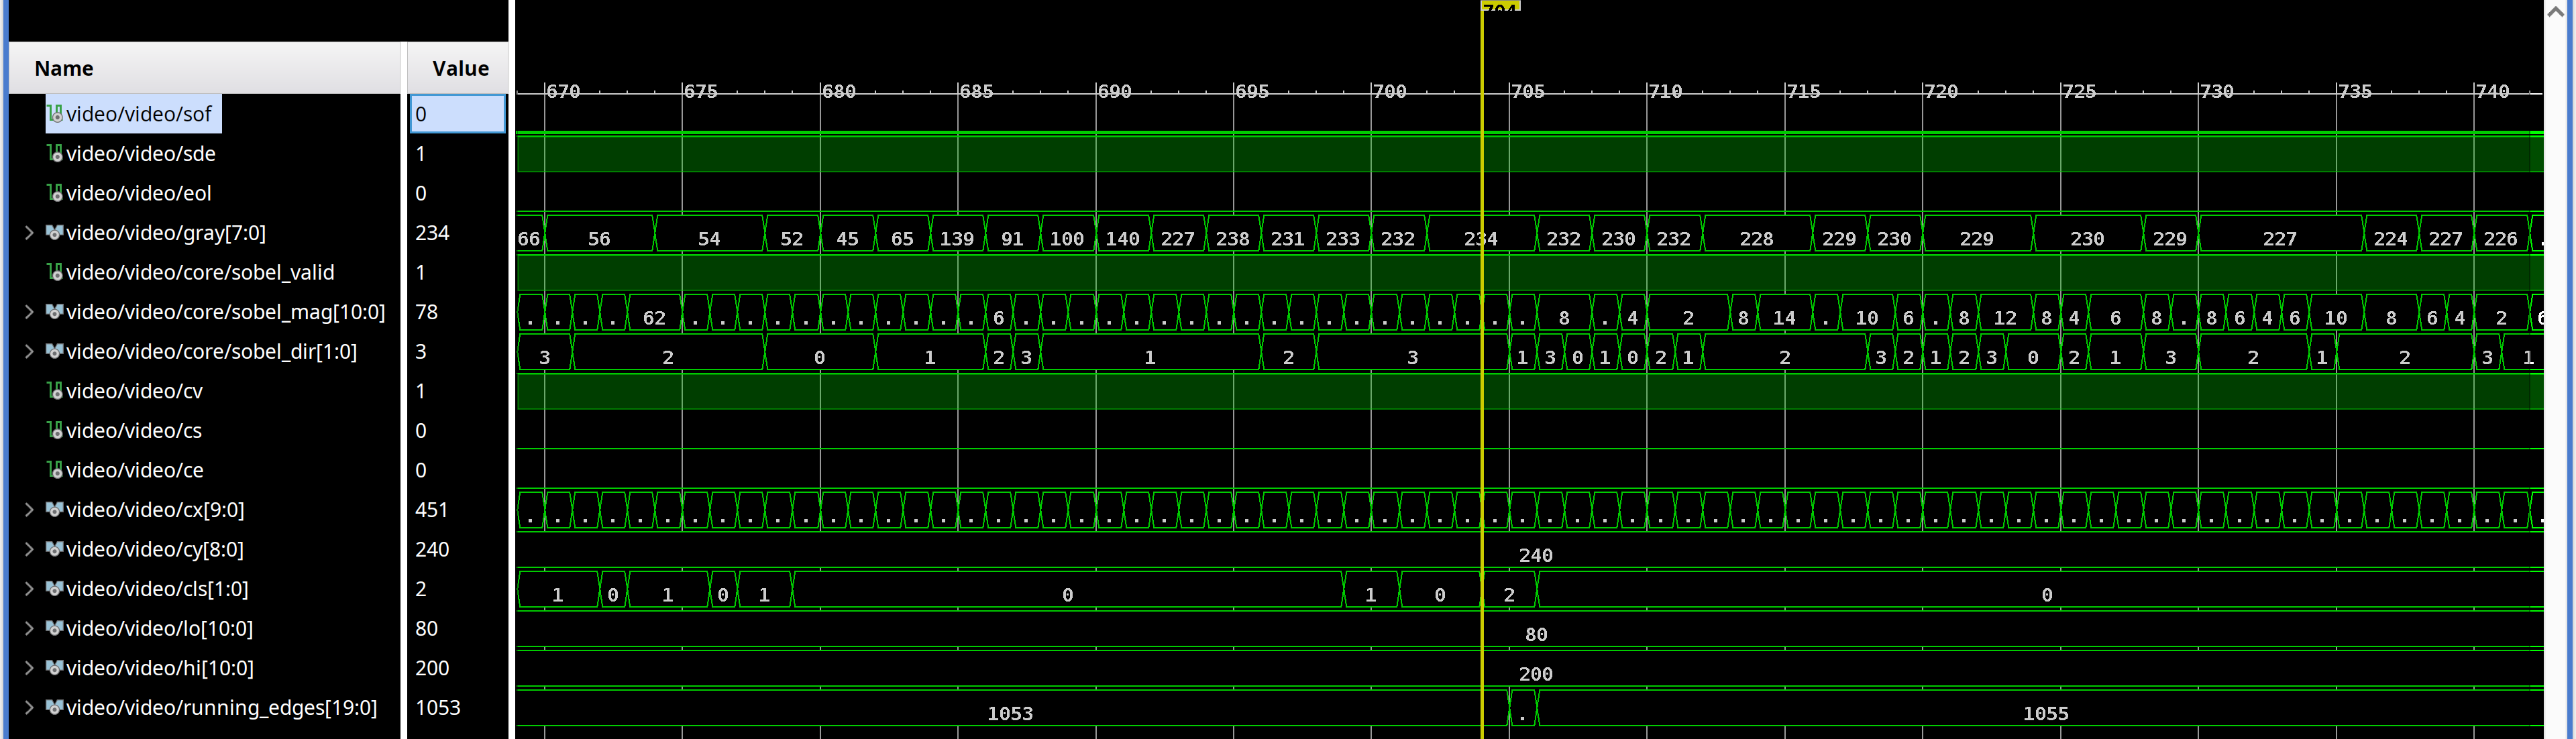
\includegraphics[width=\linewidth]{ila_fig.png}
\caption{ILA capture on the Zybo Z7-10 (Vivado hardware manager; stored photo, thresholds 80/200). The cursor (sample 704) is
on output pixel (451, 240), classified strong (\texttt{cls}=2), and \texttt{running\_edges} counts it (1053$\to$1055 over two strong
pixels). Each probe sits at its own pipeline stage, so one column shows different pixels at input, Sobel and output.}\label{fig:ila}
\end{figure}
\textbf{Demo.} The monitor shows the original, smoothed, strong-edge and class views selected by SW1:0 (Fig.~\ref{fig:demo} in Appendix~\ref{app:demo}); SW3:2
select four threshold presets; BTN2 toggles live webcam mode, in which the laptop webcam is processed live.

%% =====================================================================
\section{Discussion and Limitations}
\label{sec:discussion}
\textbf{What worked.} Writing the golden model first and comparing every stage at its raster position found all RTL bugs before
hardware (the one problem seen only on the board was in the firmware); the line buffer carries coordinates with the data, so gaps and blanking never break alignment. Formal checking was most useful on
the controller: the hand labelling and NuSMV showed that a liveness property needs a fairness assumption, and one property
turned out to be wrong in the specification, not in the RTL. \textbf{What did not, or differently from the card.} (1) The board has HDMI, not VGA; the output uses VGA (VESA DMT)
timing over DVI. (2) No DDR/DMA and no OV7670: frames come from BRAM over JTAG or from the laptop webcam over HDMI-in at 320$\times$240
(shown 2$\times$). (3) No interrupt; the firmware polls once per frame. (4) The paper-enhanced design is verified and synthesised but not
yet in the bitstream. (5) Post-route SDF timing simulation of the HDMI transmitter was not completed (static timing passes). (6)
NuSMV proofs of \texttt{vga\_timing} use reduced sizes (SymbiYosys covers the real size); quality figures are for six images and two
references only. \textbf{Lesson.} The ``fewest operators'' HLS design point was the largest on the FPGA: on LUT fabrics
multiplexers are as expensive as small adders, so the pipelined II$=$1 datapath is both the fastest and the smallest here.

%% =====================================================================
\section{Conclusion and Future Work}
\label{sec:conclusion}
We built and verified a 640$\times$480@60\,Hz, one-pixel-per-clock Canny-style pipeline: 2{,}108 LUT, 3 BRAM tiles and no DSP for the
core, 3 lines of latency, 437$\times$ faster than software on the same RV32 core, bit-exact with the golden model on 29.8 million
pixels, with 13 assertions, 25 CTL properties and three k-induction proofs, running live on the Zybo Z7-10. Incorporating Guo and Wu's
adaptive Otsu threshold in streaming form removed the paper's 80-RAMB36 frame buffer at the cost of one BRAM tile and 10 DSPs, with
thresholds identical to the paper's engine and a strong-edge F1 that rises from 0.41 to 0.83.
\textbf{Future work:} (i) put the streaming Otsu unit into the board build behind a switch and pipeline its log unit; (ii) use the
Zynq PS with AXI VDMA for full-resolution 640$\times$480 frames from DDR and an interrupt on frame end.

%% =====================================================================
\section*{Contribution Statement and Acknowledgements}
\addcontentsline{toc}{section}{Contribution Statement and Acknowledgements}
\label{sec:contrib}
\begin{table}[H]\centering\footnotesize
\begin{tabularx}{\linewidth}{@{}lX@{}}
\toprule
Member & Main contributions\\
\midrule
\studentA & Main RTL core (line buffers, Gaussian, Sobel, NMS, classifier/histogram, APB), video/HDMI path and board tops,
RV32 SoC and firmware, FPGA bring-up on both boards and the live-webcam mode, regression and verification infrastructure.\\
\studentB & Independent golden model, Espresso study of the direction block, research-paper RTL and quality study, abstract CTL
model of the controller with mutants, hand-HLS derivation of the Sobel CSE form.\\
Both & Merging the two trees; the final analyses of this report (scheduling/binding and FSMD design points, streaming Otsu unit,
FSM minimisation/encoding, QM/UCP, BDD, SymbiYosys, SVA/coverage). Both members can explain every part.\\
\bottomrule
\end{tabularx}
\end{table}
\textbf{Open-source IP used:} PicoRV32 RV32I core (C.~Wolf, ISC licence); Digilent \texttt{rgb2dvi} and \texttt{dvi2rgb} HDMI IP (BSD-style;
\texttt{dvi2rgb} locally extended with a debug port); the paper's adaptive-threshold reference RTL (\texttt{rtl/study/paper}, used as
supplied); Berkeley ESPRESSO, PyEDA, \texttt{dd}, NuSMV 2.6, Yosys/ABC, SymbiYosys with z3, Verilator, Icarus Verilog.\\
\textbf{AI-tool use:} Claude Code (Anthropic) was used extensively as a programming and analysis assistant: debugging RTL; writing and debugging
testbenches and analysis scripts, running the tool flows, and drafting parts of this report. Every number in the report is produced by a
script or tool log in the repository; we reviewed the design decisions and results and take responsibility for them.

%% =====================================================================
\begin{thebibliography}{99}\small
\bibitem{canny} J. Canny, ``A computational approach to edge detection,'' \emph{IEEE Trans. Pattern Anal. Mach. Intell.}, vol.~PAMI-8,
  no.~6, pp.~679--698, 1986, doi:10.1109/TPAMI.1986.4767851.
\bibitem{vesa} VESA, \emph{VESA and Industry Standards and Guidelines for Computer Display Monitor Timing (DMT)}, ver.~1.0, rev.~13, 2013.
\bibitem{xu2014} Q. Xu, S. Varadarajan, C. Chakrabarti and L. J. Karam, ``A distributed Canny edge detector: algorithm and FPGA
  implementation,'' \emph{IEEE Trans. Image Process.}, vol.~23, no.~7, pp.~2944--2960, 2014, doi:10.1109/TIP.2014.2311656.
\bibitem{he2008} W. He and K. Yuan, ``An improved Canny edge detector and its realization on FPGA,'' in \emph{Proc. 7th World Congress
  on Intelligent Control and Automation (WCICA)}, 2008, pp.~6561--6564.
\bibitem{otsu} N. Otsu, ``A threshold selection method from gray-level histograms,'' \emph{IEEE Trans. Syst., Man, Cybern.}, vol.~9,
  no.~1, pp.~62--66, 1979, doi:10.1109/TSMC.1979.4310076.
\bibitem{guo2023} L. Guo and S. Wu, ``FPGA implementation of a real-time edge detection system based on an improved Canny algorithm,''
  \emph{Applied Sciences}, vol.~13, no.~2, art.~870, 2023, doi:10.3390/app13020870.
\bibitem{demicheli} G. De Micheli, \emph{Synthesis and Optimization of Digital Circuits}. McGraw-Hill, 1994.
\bibitem{bening} L. Bening and H. Foster, \emph{Principles of Verifiable RTL Design}, 2nd ed. Kluwer, 2001.
\bibitem{espresso} R. K. Brayton, G. D. Hachtel, C. T. McMullen and A. L. Sangiovanni-Vincentelli, \emph{Logic Minimization Algorithms
  for VLSI Synthesis}. Kluwer, 1984.
\bibitem{bryant} R. E. Bryant, ``Graph-based algorithms for Boolean function manipulation,'' \emph{IEEE Trans. Comput.}, vol.~C-35,
  no.~8, pp.~677--691, 1986.
\bibitem{rudell} R. Rudell, ``Dynamic variable ordering for ordered binary decision diagrams,'' in \emph{Proc. ICCAD}, 1993, pp.~42--47.
\bibitem{picorv32} C. Wolf, ``PicoRV32 -- a size-optimized RISC-V CPU,'' \url{https://github.com/YosysHQ/picorv32}.
\end{thebibliography}

%% =====================================================================
\appendix
\section{Repository and How to Reproduce}
\label{app:repro}
Repository: \url{\repourl}. Layout: \texttt{rtl/} core and board RTL, \texttt{rtl/study/} paper, baseline, FSMD and enhanced designs,
\texttt{tb/} testbenches (\texttt{tb/sva} assertions), \texttt{model/} golden model, \texttt{hls/}, \texttt{logic/}, \texttt{formal/}
analyses, \texttt{fw/} firmware, \texttt{scripts/} flows, \texttt{fpga/} constraints, \texttt{docs/} guides (demo, Vivado GUI flow).
\begin{lstlisting}[language=bash,numbers=none]
make verify                                    # unit, stress, core regression, video, SoC, CTL (vga_timing, ctrl_sync)
python scripts/sva_coverage.py                 # SVA bind + Verilator line/toggle coverage + assertion mutant
python hls/sobel_hls.py                        # transformations, ASAP/ALAP, list scheduling, ILP, binding, FSMD RTL
python logic/logic_study.py                    # implication chart, encoding heuristic, QM/UCP, ESPRESSO, kernels, ABC
python scripts/ooc_batch.py <jobs.json> <out>  # Vivado OOC numbers (design points, encodings, enhanced design)
python formal/otsu_ctl.py                      # NuSMV CTL + fairness on otsu_ctrl, bug injection, simulation replay
python formal/bdd_study.py                     # BDD orderings, sifting, equivalence, symbolic reachability
python formal/run_sby.py                       # SymbiYosys BMC + k-induction
python scripts/otsu_stream_check.py            # streaming Otsu vs. the paper's engine (6 images, 640x480)
make study                                     # paper / baseline quality and resource comparison
P7_BOARD=zybo_z7 vivado -mode batch -source scripts/build_hdmi.tcl ; make live   # bitstreams
make ila ; vivado -mode gui -source scripts/ila_capture.tcl -tclargs capture 240  # ILA build + capture (Fig. 6)
\end{lstlisting}

\section{Additional Material}
\subsection{Raster-timing CTL results (shipped RTL, NuSMV)}
\label{app:ctl}
\texttt{vga\_timing} (instance H\_TOTAL$=$6, V\_TOTAL$=$5): P1 $h<H_\text{TOTAL}$, P2 $v<V_\text{TOTAL}$, P3 SOF only at the origin,
P4 $\mathbf{AG\,EF}\,\mathit{sof}$, P5 $\mathbf{AG\,EF}\,\mathit{eof}$, P6 EOL$\Rightarrow$DE, P7 line wrap ($\mathbf{AX}$), P8 frame wrap,
P9 $\mathbf{AG\,EF}\,\mathit{de}$, P10 EOF$\Rightarrow$EOL: all true, transition relation total. Mutants (line one clock too long; frame
never wraps; SOF late; EOL late; vertical counter stuck) are caught by P1/P7/P8, P8, P3, P6 and P5. \texttt{ctrl\_sync} (3$\times$3):
out-of-range coordinate raises \emph{sync\_error}, $\mathbf{AG\,EF}$ clean stream, $\mathbf{AG\,EF}$ frame start: all true; 3 mutants caught.

\subsection{Paper engine: log-domain Otsu vs.\ floating-point Otsu}
\label{app:paper}
\begin{table}[H]\centering\small
\begin{tabular}{@{}lcccccc@{}}
\toprule
Image & camera & astronaut & coins & coffee & chelsea & rocket\\
\midrule
$T_\text{hi}$ (paper RTL = our streaming unit) & 102 & 110 & 98 & 84 & 46 & 80\\
Exact Otsu $k$ (float; class 0 $=\{\le k\}$) & 102 & 102 & 94 & 88 & 44 & 76\\
Difference to $k$ or $k{+}1$ (levels) & 0 & 7 & 3 & 4 & 1 & 3\\
\bottomrule
\end{tabular}
\end{table}
Because the float threshold separates $k$ from $k{+}1$, the difference is taken to the nearer of the two. The differences (0--7 levels) come from the 16-segment piecewise-linear $\log_2$ approximation of the paper's unit.

\subsection{NuSMV model of the controller (excerpt of the property file)}
\begin{lstlisting}[language=SMV]
MODULE main
VAR top : _otsu_ctrl;                 -- Yosys write_smv of rtl/otsu_ctrl.sv, inputs as free variables
INVAR top._rst = 0ub1_0
INIT top._state = 0ub3_000            -- INIT
FAIRNESS bool(top._odone)
FAIRNESS bool(top._cdone)
FAIRNESS bool(top._eof)
FAIRNESS (bool(top._en) & bool(top._sof))
CTLSPEC AG (bool(top._swap) -> AX AF (bool(top._apply) | top._state = 0ub3_000));
\end{lstlisting}

\subsection{Board demonstration views}\label{app:demo}
\begin{figure}[H]\centering
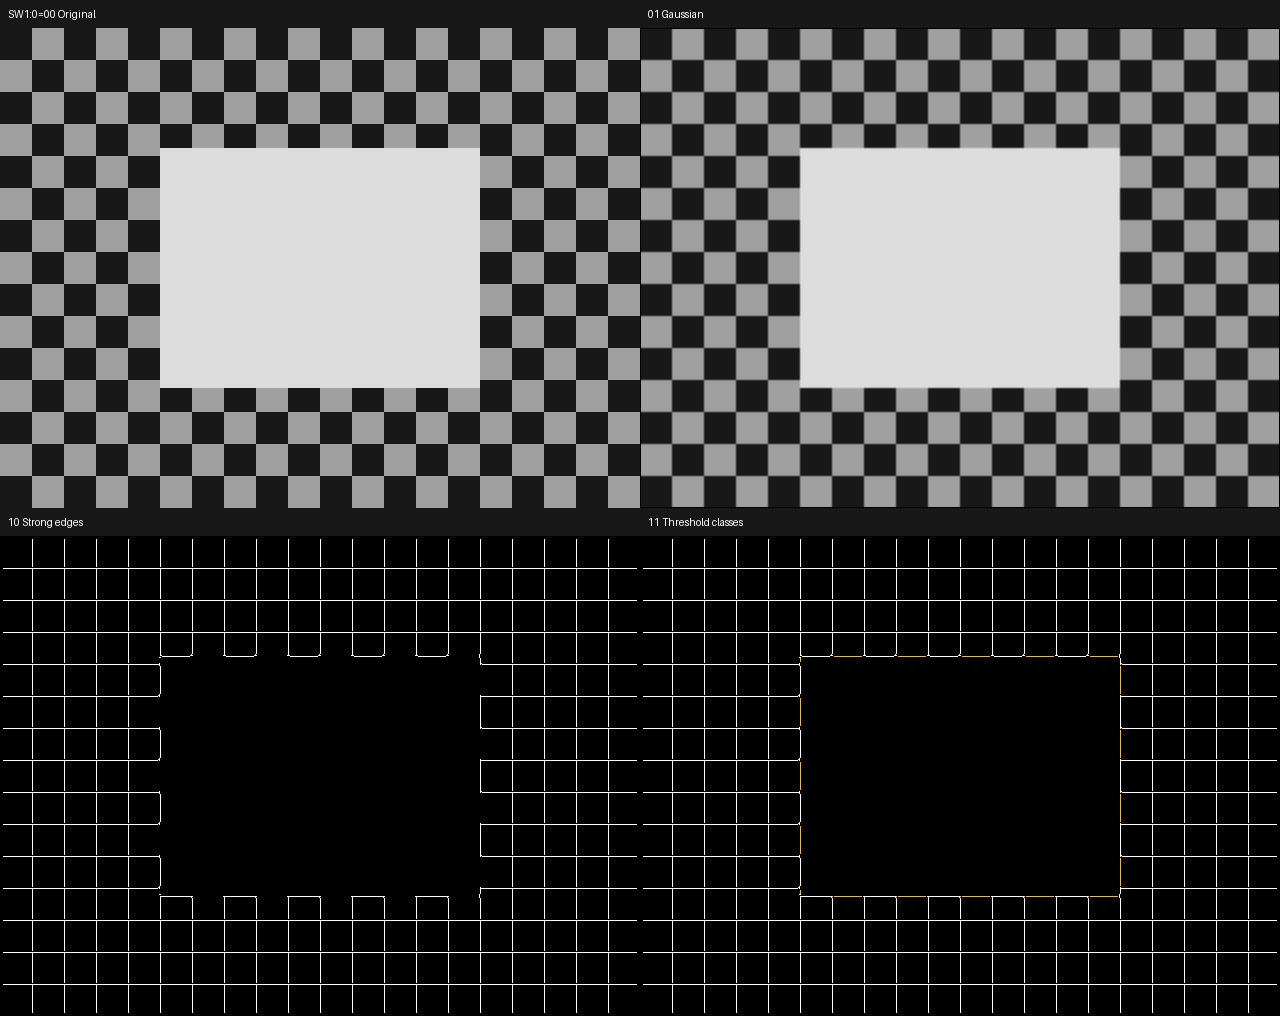
\includegraphics[width=0.30\linewidth]{views.png}\hspace{4mm}
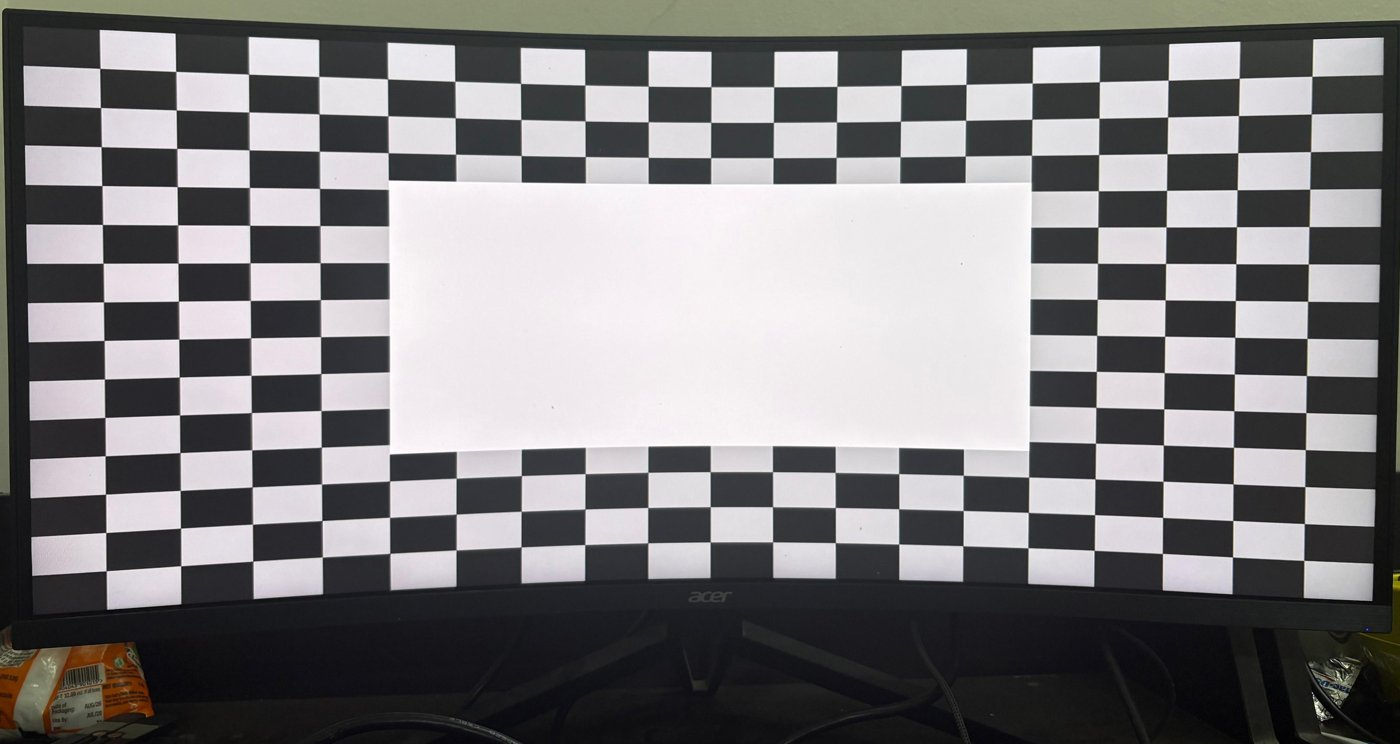
\includegraphics[width=0.42\linewidth]{monitor.jpg}
\caption{Left: the four views of the board design in the routed-netlist simulation (original, smoothed, strong edges, classes).
Right: the Zybo Z7-10 driving the monitor at 640$\times$480 over HDMI (original view of the test pattern).}\label{fig:demo}
\end{figure}

\end{document}
